\documentclass{article}
\usepackage[english]{babel}
\usepackage{amsthm}
\usepackage{amsmath}

\newtheorem{theorem}{Theorem}[section]
\newtheorem{corollary}{Corollary}[theorem]
\newtheorem{lemma}[theorem]{Lemma}
% \newtheorem{observation}[theorem]{Observation}
\newtheorem{observation}[theorem]{Observation}
\newtheorem{claim}[theorem]{Claim}
\newtheorem{exercise}{Exercise}


\usepackage[utf8]{inputenc}
\usepackage{graphicx}
\graphicspath{{images/}}


\usepackage{tikz}
\usetikzlibrary{calc,tikzmark}

\begin{document}
\section{Friendship Graphs}
A \textbf{friendship graph} $F_n$ is a planar, undirected graph with $2_n + 1$ vertices and $3n$ edges. The friendship graph can be constructed by joining $n$ copies of the cycle $C_3$ with a common vertex, which becomes the \textbf{universal vertex} for the graph.  

\begin{figure}[htp]
    \centering
    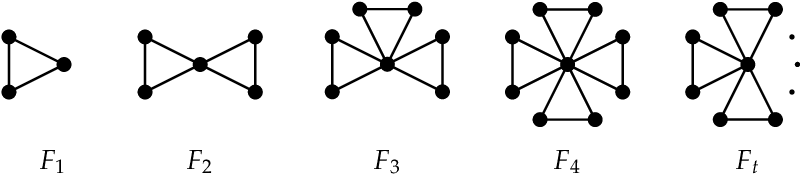
\includegraphics[width=8cm]{friendship_graphs.png}
    \label{fig:friendship_graphs}
\end{figure}

\begin{theorem}[Friendship Theorem]
\label{theorem:friendship}
Let $G$ be a finite graph such that every pair of vertices have exactly one common neighbor. Then $G$ has a vertex adjacent to every other vertex, (a universal vertex).
\end{theorem}


\begin{proof}
\label{proof:friendship_theorem}
Suppose to the contrary that each pair of vertices in $G$ has a common neighbor but no universal vertex. Following from the common neighbor property as stated in \ref{theorem:friendship}, we observe the following:

\begin{observation}
$G$ has no 4-cycles, as any pair of vertices on a $C_4$ would have two common neighbors. 
\end{observation}

From this observation we make the following claim:

\begin{claim}
\label{claim:regularity}
$G$ is a regular graph.
\end{claim}

Begin with non-adjacent vertices $u, v \in G$ via no universal vertex. There must be exactly one common vertex between $u$ and $v$, i.e. this common vertex must be contained in $N(u) = \{w_1, w_2, ... , w_k\}$. Say WLOG this common vertex is $w_2$. There must also be exactly one common vertex between $u$ and $w_2$. Say WLOG this common vertex is $w_1$. We take notice of the following:

\begin{enumerate}
    \item $v$ is not adjacent to any $w_i$ (where $i \neq 2$)
    \item No pair of $w_i, w_j$ have a common neighbor other than $u$
    \item $v, w_i$ have a common neighbor (where $ i \geq 2$)
\end{enumerate}

From these observations we conclude $d(u) \geq d(u)$. We can symmetrically argue $d(v) \geq d(u)$. Combining both conclusions we have $d(u) = d(v) = k$. From here we make the following observation:

\begin{observation}
\label{obs:adjacency}
Every vertex $x$ (except $w_2$) is \textbf{not} adjacent to $u$ or $v$. Hence, $d(x) = k$.
\end{observation}  

Since $w_2$ is not universal (as stated in the aim of the proof), there is some vertex $y$ to which $w_2$ is not adjacent. But from our observation \ref{obs:adjacency}, $d(y) = k$. Thus, $d(w_2) = k$, which proves the claim \ref{claim:regularity}. 

\bigskip

The regularity of $G$ allows the conclusion that the sum of degrees for 
$w_1, w_2, ..., w_k = k^2$. Notice that this sum counts every vertex of $G$, as every vertex in $G$ has a common neighbor with $u$, so this common neighbor must exist as $w_i$ (and is not repeated). Further, $u$ is counted $k$ times for each of its $k$ edges. Thus we can deduce $|V(G)| = n = k^2 - k + 1$.

We can then make the following observation: 
\begin{observation}
\label{obs:kgr2}
We know $k > 2$, as
\[
k = 1 \rightarrow n = 1
\]
\[
k = 2 \rightarrow n = 3
\]

\end{observation}  

\bigskip

Let us consider the adjacency matrix $A$ of $G$ and its square, $A^2$

\begin{figure}[ht]
\centering
$A = $
    $\begin{bmatrix}
        0         & a_{01}      & \dots     & a_{0j}       \\
        a_{10}    & 0           & \dots     & \dots        \\
        \vdots    & \vdots      & \ddots    & \dots        \\
        a_{i0}    & \hdots      & \hdots    & 0.           \\
    \end{bmatrix}$
\[
    a_{ij}= 
\begin{cases}
    1, & \text{if } $ v_i v_j$ is an edge \\
    0,              & \text{otherwise}
\end{cases}
\]
\end{figure}

We can leverage $A$ toward a contradiction by considering the following property of $A^2$:

\begin{theorem}
\label{theorem:adjacency}
$A^2$ counts the number of walks of length 2 in $G$.
\end{theorem}

\begin{figure}[ht]
\centering
$A^2 = $
    $\begin{bmatrix}
        k         & 1           & \dots     & 1         & 1       \\
        1         & k           & \dots     & \dots     & 1    \\
        \vdots    & \vdots      & \ddots    & \dots     & \dots    \\
        1         & \hdots      & \hdots    & k         & 1      \\
        1         & 1           & \hdots    & 1        & k      \\
    \end{bmatrix}$
\[
    a^2_{ij}= 
\begin{cases}
    k, & \text{if } $$v_i = v_j$$ \\
    1,              & \text{otherwise}
\end{cases}
\]
\end{figure}

When $v_i \neq v_j$ we know each $v_iv_j$ pair has exactly one walk of length 2. And when $v_i = v_j$, the number of walks is simply the degree of the vertex, as a length-two walk simply travels along one out-edge return on the same edge for each of its $k$ out-edges.

Written another way, $A^2 = J + (k - 1)I$, where $J$ is the ones-matrix and $I$ is the identity matrix. 
Computing the eigenvalues of $A^2$ gives:


\[ \lambda = 
    \left (
        \begin{array}{c}
            \
            k - 1 + n = k^2 \tikzmark{lineOne} \\
            k - 1 \tikzmark{lineTwo}\\
            \vdots \\
        \end{array}
    \right )
\]

\begin{tikzpicture}[overlay,remember picture]
\node[anchor=west] at ($(pic cs:lineOne)+(.7,.1)$) {\small $\gets$ multiplicity of $1$};
\node[anchor=west] at ($(pic cs:lineTwo)+(1.5,.1)$) {\small $\gets$ multiplicity of $n-1$};

\end{tikzpicture}

Note that $k - 1 + n$ is indeed $k^2$ as we concluded from \ref{obs:adjacency}. We can simply calculate the element-wise square root of $A^2$'s eigenvalues of to determine the eigenvalues of $A$:

\[ \lambda = 
    \left (
        \begin{array}{c}
            \
            \sqrt{k^2} = k \tikzmark{lineOneb} \\
            \pm \sqrt{k - 1} \tikzmark{lineTwob}\\
            \vdots \\
        \end{array}
    \right )
\]

\begin{tikzpicture}[overlay,remember picture]
\node[anchor=west] at ($(pic cs:lineOneb)+(1.1,.1)$) {\small $\gets$ multiplicity of $1$};
\node[anchor=west] at ($(pic cs:lineTwob)+(1.1,.1)$) {\small $\gets$ multiplicity of $n-1$};

\end{tikzpicture}

We unpack the $\pm \sqrt{k-1}$ and restate the values and multiplicities the following way:

\[ \lambda = 
    \left (
        \begin{array}{c}
            \
            \sqrt{k^2} = k \tikzmark{lineOnec} \\
            + \sqrt{k - 1} \tikzmark{lineTwoc}\\
            \dots \\
            - \sqrt{k - 1} \tikzmark{lineThreec}\\
            \vdots \\
        \end{array}
    \right )
\]

\begin{tikzpicture}[overlay,remember picture]
\node[anchor=west] at ($(pic cs:lineOnec)+(1.1,.1)$) {\small $\gets$ multiplicity of $1$};
\node[anchor=west] at ($(pic cs:lineTwoc)+(1.1,.1)$) {\small $\gets$ multiplicity of $r$};
\node[anchor=west] at ($(pic cs:lineThreec)+(1.1,.1)$) {\small $\gets$ multiplicity of $s$};

\end{tikzpicture}

Summing the eigenvalues of $A$ gives $k + r\sqrt{k - 1} - s\sqrt{k -1}$. This value is equivalent to summing the diagonal of $A$, which is a property of eigenvalues we can now exploit. Recall $A$'s diagonal is all 0's, which gives:

\[ 
k + r\sqrt{k - 1} - s\sqrt{k -1} = 0
\]

Refactoring above and multiplying $k$ throughout results in the following:

\[
(r - s)(k - 1) = k^2
\]

This implies that $(k - 1)$ divides $k^2$, which only happens if $k \leq 2$ which contradicts observation \ref{obs:kgr2}.

\end{proof}

\end{document}